\documentclass[crop,border=5,tikz,convert={outext=.svg,command=\unexpanded{pdf2svg
    \infile\space\outfile}},multi=false]{standalone}
\usetikzlibrary{math,calc,through,shapes,patterns}
\usepackage{graphicx}
\usepackage{subcaption}

\newcommand{\markangle}[6][0.25]{
  \begin{scope}
    \clip (#2)--(#3)--(#4);
    \node (ANG) [draw, circle, minimum size=#5] at (#3){};
  \end{scope}
  \coordinate (E1) at (intersection 0 of ANG and #3--#2);
  \coordinate (E2) at (intersection 0 of ANG and #3--#4);
  %\draw[thick] (E1) to [bend right=50] (E2);
  \coordinate (EM) at ($ (E1)!0.5!(E2) $);
  \coordinate (EM) at ($ (EM)!#1!(#3) $);
  \node at (EM) {#6};
}



\begin{document}


\begin{figure}[!h]
\centering
\begin{subfigure}[b]{0.45\textwidth}
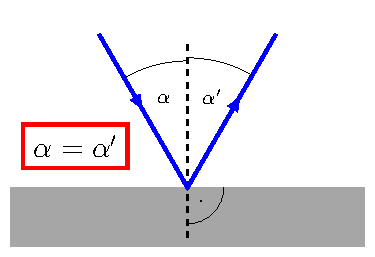
\includegraphics[scale=1]{rlaw1.ps}
\caption{Total Reflection}
\end{subfigure}
~
\begin{subfigure}[b]{0.45\textwidth}
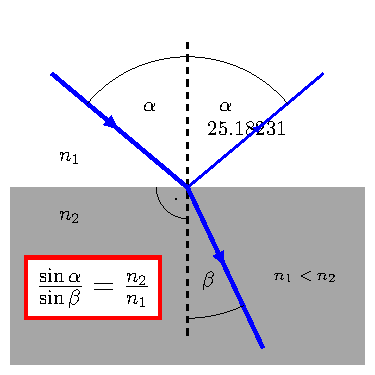
\includegraphics[scale=1]{rlaw2.ps}
\caption{TODO}
\end{subfigure}

\begin{subfigure}[b]{0.45\textwidth}
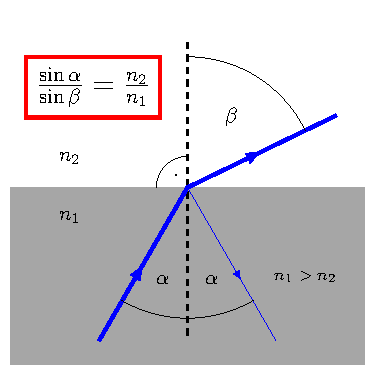
\includegraphics[scale=1]{rlaw3.ps}
\caption{TODO}
\end{subfigure}
~
\begin{subfigure}[b]{0.45\textwidth}
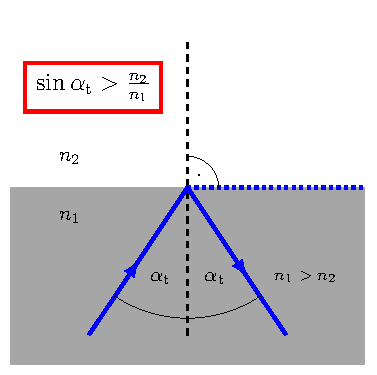
\includegraphics[scale=1]{rlaw4.ps}
\caption{TODO}
\end{subfigure}

\caption{Cases of light through Ovio Slit.}
\end{figure}

\end{document}
